\documentclass[12pt]{article}

\usepackage{tema2014}

\usepackage{graphicx,url}

\usepackage[brazil]{babel}
\usepackage[utf8]{inputenc}


\sloppy

\title{Modelo de documento para as conferências da TeMA}

\author{Marcos da Silva Sampaio\inst{1}, Guilherme Bertissolo\inst{1}, Alexandre Espinheira\inst{1}}

\address{Grupo de Pesquisa Genos ---
         Escola de Música da Universidade Federal da Bahia \\
         Av. Araújo Pinho, 58 ---
         40110-913 Salvador, BA
         \email{marcos@sampaio.me, guilhermebertissolo@gmail.com, alespinheira@gmail.com}
}

\begin{document}

\maketitle

\begin{abstract}
  This meta-paper describes the style to be used in paper submission
  for the conferences of Associação Brasileira de Teoria e Análise
  Musical (TeMA).
\end{abstract}

\keywords{Template, TeMA, Music, Conference}

\begin{resumo}
  Este meta-artigo descreve o estilo a ser usado na elaboração de
  artigos para submissão nas conferências da Associação Brasileira de
  Teoria e Análise Musical (TeMA).
\end{resumo}

\palavraschave{Modelo, TeMA, Música, Congresso}

\section{Introdução}
\label{sec:gen}

Este modelo inclui toda a informação referente à formatação de artigos
para as conferências da TeMA. Este guia deverá ser seguido para que os
anais dos eventos tenham um padrão uniforme. Este modelo pode ser
obtido na página da TeMA (http://tema.mus.br).


\section{Tamanho da página}
\label{sec:tamanho-pagina}

Os anais serão organizados em formato A4 retrato (21.0cm x 29.7cm).
Todo o conteúdo de cada página deverá caber dentro do retângulo de
17cm x 25.2cm, centralizado na página, com margens 2cm (topo), 2.5cm
(base), 2cm (esquerda/direita). O texto deverá estar inteiramente
justificado, com separação de sílabas.

\section{Fonte}
\label{sec:fonte}

Todo o texto deverá ter fonte Times, exceto pelas legendas das figuras
(vide seção~\ref{sec:figuras-e-tabelas}). Fontes sem serifa e não
proporcional só podem ser usadas com propósitos especiais, como para
diferenciar texto de código-fonte de programas.

\section{Primeira página}

A primeira página deverá conter o título do artigo, o nome e endereço
dos autores, o abstract e \textit{keywords} em inglês, e, nos textos
em português, o resumo e palavras-chave.

\subsection{Título}
\label{sec:titulo}

O título deverá ser centralizado sobre a página, com fonte Times em
negrito 16pt. O espaçamento entre \textit{keywords} e resumo deverá
ser de 6pt.

\subsection{Autores}
\label{sec:autores}

Os nomes dos autores são omitidos na submissão para revisão. Para a
versão final, deverão estar centralizados, com fonte Times 12pt, em
negrito, todos dispostos em uma mesma linha, separados por vírgulas.
Os endereços deverão estar centralizados, com fonte Times 12pt. Se o
endereço dos autores for o mesmo, deverá ser inserido apenas uma vez,
centralizado. Se os endereços forem diferentes, deverão ser espaçados,
sob os nomes dos autores.

\subsection{Abstract e resumo}
\label{sec:abstract-e-resumo}

O abstract e o resumo deverão ter fonte Times itálico 12pt, em
itálico, indentado em 0.8cm em ambos os lados. O espaçamento entre
\textit{abstract}, \textit{keywords}, resumo e palavras-chave deverá
ser de 6pt.

O resumo deverá conter uma introdução, o objetivo do projeto
trabalhado, a metodologia, os resultados (parciais ou finais) e
apontar as conclusões. O resumo deverá ter, no máximo de 250 palavras,
sem parágrafo e sem citações bibliográficas.

\subsection{\textit{Keywords} e palavras-chave}
\label{sec:keywords-e-palavras}

O texto deverá conter até 5 \textit{keywords} e palavras-chave
separadas por vírgula.

\section{Corpo do texto}

\subsection{Seções e subseções}
\label{sec:secoes}

Os títulos de seções e subseções deverão ser obrigatoriamente
enumerados, deverão ter fonte Times, negrito, 13pt e alinhamento à
esquerda.

Títulos de seções e subseções deverão ser precedidos e sucedidos de
espaço extra. Em seções os títulos deverão ser precedidos por espaço
de 12pt, e em subseções, 6pt. Ambos deverão ser sucedidos por espaço
de 6pt.

\subsection{Parágrafos}
\label{sec:paragrafos}

O primeiro parágrafo de cada seção não deverá estar indentado. Os
seguintes deverão ter indentação 0.5cm. O espaçamento entre parágrafos
deverá ser de 3pt.

\subsection{Números de página, cabeçalhos e rodapés}

As páginas não deverão conter cabeçalhos, rodapés ou números de página
em sua submissão. Estes elementos serão adicionados quando os anais
forem confeccionados.

\subsection{Notas de rodapé}

As notas de rodapé deverão ser identificadas com um número no texto e
inseridas na base da página em que aparecem\footnote{Este é um exemplo
  de nota de rodapé.}. As notas deverão ter fonte de 8pt e deverão ser
precedidas de linha horizontal de 0.5pt.

\section{Figuras e tabelas}
\label{sec:figuras-e-tabelas}

As figuras e tabelas deverão ser, preferencialmente, flutuantes,
ocorrendo no topo da página em que são mencionadas ou da página
seguinte. Figuras e tabelas deverão ser enumeradas
\textbf{independentemente} e referendadas por seus números (por
exemplo, figura~\ref{fig:exampleFig}).

\begin{figure}
\centering
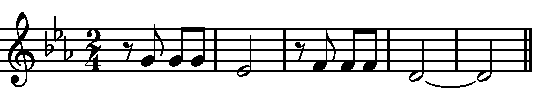
\includegraphics[width=.5\textwidth]{beethoven}
\caption{Uma figura típica}
\label{fig:exampleFig}
\end{figure}

As legendas das figuras e tabelas, se menores que uma linha, deverão
ser centralizadas). Nos outros casos, deverão ser justificadas e
indentadas em 0.8cm em ambos lados. A fonte deverá ser Helvetica
negrito, de 10pt, com 6pt de espaço antes e depois de cada legenda.

Nas tabelas, não usar fundo colorido ou sombreado e evitar linhas
grossas, duplas ou desnecessárias.


\section{Imagens}

Todas as imagens e ilustrações deverão estar em preto e branco ou tons
de cinza. A resolução das imagens deverá ser de até 600 dpi para preto
e branco e 200 dpi para tons de cinza. Não incluir imagens com
resolução excessiva.

\section{Referências}

Referências bibliográficas deverão ser uniformes, com o sistema
Turabian autor data. Por exemplo, \cite{kroger04:desenvolvendo},
\cite{babbitt61:set}, \cite{coutinho.ea05:computational},
\cite{morris87:composition}.

\bibliography{example}

\end{document}
